\section{Real-Time Scheduling}
\label{sec:sched}


  We now provide a brief overview of real-time scheduling under auditing using the two representative timelines given in Figure~\ref{fig:timelines}.
  The baseline scenario shows execution timeline for two periodic tasks that are not under audit.
  Audit overheads can be divided into two parts: (i)
  part  $A(\cdot)$ represents the task execution with additional synchronous overhead of log generation and  (ii) part 
  $B(\cdot)$ represents the processing time required to maintain  the audit logs, transporting them from kaudit buffer to userspace and eventually to persistent storage (as shown in Figure~\ref{fig:audit_arch}).
  Audit log maintenance (Task $B(\cdot)$) is composed of \texttt{kauditd} and \texttt{auditd} daemons that run with background priority. 
  
  Task $B(\cdot)$ varies with the number of log events that need to be maintained.
  Any additional overheads of log maintenance, like transporting them to a remote server can also be trivially included in this component.

  \begin{figure}[t!]
    \centering 
      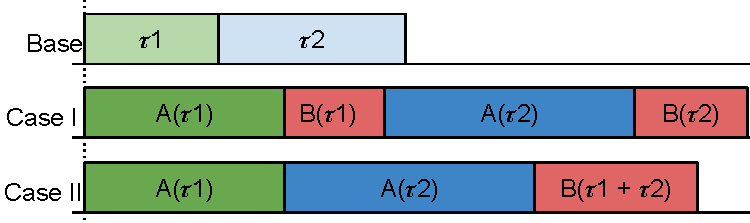
\includegraphics[width=.8\linewidth]{fig/timelines.pdf}
      \caption{\label{fig:timelines}Sample timelines for two periodic tasks. \textit{Base} is without auditing. \textit{Case I and II} show potential schedules with auditing related overheads. $A(\cdot)$ is the increased computation time of the task including audit log generation overhead. $B(\cdot)$ represents the runtime of \textit{kauditd} and \textit{auditd} daemons as they handle the logs generated by the real-time tasks.}
    \end{figure} 
  
 Depending on the scheduling algorithm, two forms of interleaving of the tasks with the audit daemons (i.e., Task $B(\cdot)$) are possible, as shown in
Figure~\ref{fig:timelines}: execute audit maintenance tasks individually with each task (Case I), or execute audit maintenance task once for all tasks (Case II).

Case I is especially suitable for memory constrained embedded systems. To provide lossless auditing the kaudit buffer only as large as the maximum number of logs generated by any one instance of any task in the task set is required.
However, Case I imposes far stringent temporal requirements for Task $B(\cdot)$, inheriting the priority of the real time task being audited.
Case II relaxes the temporal requirement, allowing Task $B(\cdot)$ to run with the lowest real-time priority. However, to provide lossless auditing, it requires a much larger kaudit buffer, large enough to store all audit logs for one hyper period of the task set.

For either scenario, we require estimates of the following metrics for computing the schedule with auditing enabled: (i) synchronous overhead of log generation and (ii) asynchronous overheads for log maintenance per system call event. Our work focuses on estimating costs associated with (ii) while prior work~\cite{Ma2018} already provides a rough estimate of synchronous overheads due to Linux Audit.